\documentclass[a4paper,twoside]{article}
\usepackage{blindtext}  
\usepackage{geometry}

% Chinese support
\usepackage[UTF8, scheme = plain]{ctex}

% Page margin layout
\geometry{left=2.3cm,right=2cm,top=2.5cm,bottom=2.0cm}


\usepackage{listings}
\usepackage{xcolor}
\usepackage{geometry}
\usepackage{amsmath}
\usepackage{float}
\usepackage{hyperref}

\usepackage{graphics}
\usepackage{graphicx}
\usepackage{epsfig}
\usepackage{float}

\usepackage{algorithm}
\usepackage[noend]{algpseudocode}

\usepackage{booktabs}
\usepackage{threeparttable}
\usepackage{longtable}
\usepackage{listings}
\usepackage{tikz}
\usepackage{multicol}

\usepackage{caption}
\usepackage{subcaption}

% cite package, to clean up citations in the main text. Do not remove.
\usepackage{cite}

\usepackage{color,xcolor}

%% The amssymb package provides various useful mathematical symbols
\usepackage{amssymb}
%% The amsthm package provides extended theorem environments
\usepackage{amsthm}
\usepackage{amsfonts}
\usepackage{enumerate}
\usepackage{enumitem}
\usepackage{listings}

\usepackage{indentfirst}
\setlength{\parindent}{2em} % Make two letter space in the first paragraph
\usepackage{setspace}
\linespread{1.5} % Line spacing setting
\usepackage{siunitx}
\setlength{\parskip}{0.5em} % Paragraph spacing setting

% \usepackage[contents =22920202204622, scale = 10, color = black, angle = 50, opacity = .10]{background}

\renewcommand{\figurename}{图}
\renewcommand{\lstlistingname}{代码} 
\renewcommand{\tablename}{表格}
\renewcommand{\contentsname}{目录}
\floatname{algorithm}{算法}

\graphicspath{ {images/} }

%%%%%%%%%%%%%
\newcommand{\StudentNumber}{22920202204622}  % Fill your student number here
\newcommand{\StudentName}{\textbf{熊恪峥}\ 肖凯欣\ 谢哲涵\ 赵淇奥}  % Replace your name here
\newcommand{\PaperTitle}{基于xv6内核的网络子系统及Socket接口实现}  % Change your paper title here
\newcommand{\PaperType}{开题报告} % Replace the type of your report here
\newcommand{\Date}{2022年10月17日}
\newcommand{\College}{信息学院}
\newcommand{\CourseName}{计算机网络与通信}
%%%%%%%%%%%%%

%% Page header and footer setting
\usepackage{fancyhdr}
\usepackage{lastpage}
\pagestyle{fancy}
\fancyhf{}
% This requires the document to be twoside
\fancyhead[LO]{\texttt{\StudentName }}
\fancyhead[LE]{\texttt{\StudentNumber}}
\fancyhead[C]{\texttt{\PaperTitle }}
\fancyhead[R]{\texttt{第{\thepage}页,共\pageref*{LastPage}页}}


\title{\PaperTitle}
\author{\StudentName}
\date{\Date}

\lstset{
	basicstyle          =   \sffamily,          % 基本代码风格
	keywordstyle        =   \bfseries,          % 关键字风格
	commentstyle        =   \rmfamily\itshape,  % 注释的风格,斜体
	stringstyle         =   \ttfamily,  % 字符串风格
	flexiblecolumns,                % 别问为什么,加上这个
	numbers             =   left,   % 行号的位置在左边
	showspaces          =   false,  % 是否显示空格,显示了有点乱,所以不现实了
	numberstyle         =   \zihao{-5}\ttfamily,    % 行号的样式,小五号,tt等宽字体
	showstringspaces    =   false,
	captionpos          =   t,      % 这段代码的名字所呈现的位置,t指的是top上面
	frame               =   lrtb,   % 显示边框
}

\lstdefinestyle{PythonStyle}{
	language        =   Python, % 语言选Python
	basicstyle      =   \zihao{-5}\ttfamily,
	numberstyle     =   \zihao{-5}\ttfamily,
	keywordstyle    =   \color{blue},
	keywordstyle    =   [2] \color{teal},
	stringstyle     =   \color{magenta},
	commentstyle    =   \color{red}\ttfamily,
	breaklines      =   true,   % 自动换行,建议不要写太长的行
	columns         =   fixed,  % 如果不加这一句,字间距就不固定,很丑,必须加
	basewidth       =   0.5em,
}

\lstdefinestyle{MakefileStyle}{
	otherkeywords={.SUFFIXES},
	morekeywords={SUFFIX, CPP_,},
	moredelim=[is][\color{mbleu}]{/*}{*/},
	morecomment=[l][commentstyle]{\#},%
	emphstyle={\color{teal}},%
	moredelim=[s][\color{teal}]{\$(}{)}%
	basicstyle=\ttfamily\scriptsize\color{black!90},%
	stringstyle=\itshape\color{magenta},%
	showstringspaces=false,%
	keywordstyle=\bfseries\color{keycolor},%
	commentstyle=\color{blue}\slshape,%
	framexleftmargin=1mm,%
	backgroundcolor=\color{black!2},%
}

\lstdefinestyle{CppStyle}{
	language        =   c++,
	basicstyle      =   \zihao{-5}\ttfamily,
	numberstyle     =   \zihao{-5}\ttfamily,
	keywordstyle    =   \color{blue},
	keywordstyle    =   [2] \color{teal},
	stringstyle     =   \color{magenta},
	commentstyle    =   \color{red}\ttfamily,
	breaklines      =   true,   % 自动换行,建议不要写太长的行
	columns         =   fixed,  % 如果不加这一句,字间距就不固定,很丑,必须加
	basewidth       =   0.5em,
}

\algnewcommand\algorithmicinput{\textbf{Input:}}
\algnewcommand\algorithmicoutput{\textbf{Output:}}
\algnewcommand\Input{\item[\algorithmicinput]}%
\algnewcommand\Output{\item[\algorithmicoutput]}%

\usetikzlibrary{positioning, shapes.geometric}

% 流程图定义基本形状
\tikzstyle{startstop} = [rectangle, rounded corners, minimum width = 2cm, minimum height=1cm,text centered, draw = black]
\tikzstyle{io} = [trapezium, trapezium left angle=70, trapezium right angle=110, minimum width=2cm, minimum height=1cm, text centered, draw=black]
\tikzstyle{process} = [rectangle, minimum width=3cm, minimum height=1cm, text centered, draw=black]
\tikzstyle{decision} = [diamond, aspect = 3, text centered, draw=black]
% 箭头形式
\tikzstyle{arrow} = [->,>=stealth]

\newtheorem{assumption}{Assumption}[section]

\begin{document}
	
%%%%%%%%%%%%%%%%%%%%%%%%%%%%%%%%%%%%%%%%%%%%
\makeatletter % change default title style
\renewcommand*\maketitle{%
	\begin{center} 
		\bfseries  % title 
		{\LARGE \@title \par}  % LARGE typesetting
		\vskip 1em  %  margin 1em
		{\global\let\author\@empty}  % no author information
		{\global\let\date\@empty}  % no date
		\thispagestyle{empty}   %  empty page style
	\end{center}%
	\setcounter{footnote}{0}%
}
\makeatother
%%%%%%%%%%%%%%%%%%%%%%%%%%%%%%%%%%%%%%%%%%%%
	
	
\thispagestyle{empty}

\vspace*{1cm}

\begin{figure}[h]
	\centering
	
\includegraphics[width=4.0cm]{logo.png}
\end{figure}

\vspace*{1cm}

\begin{center}
	\Huge{\textbf{\PaperType}}
	
	\Large{\PaperTitle}
\end{center}

\vspace*{1cm}

\begin{table}[h]
	\centering	
	\begin{Large}
		\renewcommand{\arraystretch}{1.5}
		\begin{tabular}{p{3cm} p{5cm}<{\centering}}
			姓\qquad 名 & \StudentName  \\
			\hline
			学\qquad号 & \StudentNumber \\
			\hline
			日\qquad期 & \Date  \\
			\hline
			学\qquad院 & \College  \\
			\hline
			课程名称 & \CourseName  \\
			\hline
		\end{tabular}
	\end{Large}
\end{table}

\newpage

\title{
	\Large{\textcolor{black}{\PaperTitle}}
}
	
	
\maketitle
	
\tableofcontents
 
\newpage
\setcounter{page}{1}

\begin{spacing}{1.2}

\section{选题介绍}

由6.828 Lab 6\cite{kaashoek20066}得到的灵感,我们将为xv6内核实现网络子系统以及Socket API。

6.828课程中讲授xv6内核\cite{cox2011xv6}的实现,并在实验中要求学生在称之为JOS的实验性微内核
操作系统中添加相应的功能。但事实上,xv6内核本身的结构和现代网络服务器中常常使用
的Linux和FreeBSD更为类似。因此,我们好奇,我们是否可以对xv6内核进行修改,来添加
对网络功能的支持,而不是在JOS上进行实现。这样,我们能够更好地通过实现相应的功能和
适配相应的库来加深对各种网络协议以及Socket API本身的理解。


\subsection{xv6简介}

xv6是对Dennis Ritchie's and Ken Thompson的Unix
Version 6 (v6)的重新实现。xv6与v6有大致相同的结构和代码风格,
但是使用了ANSI C实现,并且为现代的处理器功能,如对称多核心等做出了相应的适配。
它主要为MIT的操作系统教学而设计。

\subsection{lwIP简介}

lwIP\cite{dunkels2001design}是一个开源的、轻量级的TCP/IP协议栈,它是一个可移植的、可裁剪的、可靠的、高效的、低成本的TCP/IP协议栈,它可以用于嵌入式系统,如微控制器、单片机、DSP等。
lwIP最初是由Swedish Institute of Computer Science的Adam Dunkels开发,现在由开源社区开发和维护。并且被多个技术公司用于商业产品中,
如Intel/Altera, Analog Devices, Xilinx, TI, ST 和 Freescale。

\section{项目目标}

\subsection{实现网络控制器驱动程序}

为了为xv6实现网络功能,首先需要实现网络控制器的驱动程序。我们将在项目进行的过程中
依照难度和时间安排,选择以下两种方案之一:

\begin{itemize}
	\item \textbf{VirtIO网络控制器 }:VirtIO\cite{russell2008virtio}是一种虚拟化设备标准,它允许虚拟机和宿主机之间的通信。VirtIO网络控制器是VirtIO标准的一部分,它允许虚拟机通过VirtIO网络控制器与宿主机进行通信。
	VirtIO具有标准化、对于虚拟机而言性能相对较好的特点。同时VirtIO的文档详尽易读。但目前VirtIO网络控制器驱动程序的参考实现较少。
	\item \textbf{E1000网络控制器 }:Qemu、Bochs和VirtualBox都支持该型网络控制器的模拟。目前为止,有很多类似的项目都实现该型网络控制器的驱动程序。但我认为它的实现相对繁琐,因此是备选方案。
\end{itemize}

我们在客观条件允许的情况下,将选择VirtIO网络控制器驱动程序的实现方案。

\subsection{移植lwIP}

6.828 Lab 6为JOS准备了lwIP的移植。而JOS与xv6虽然大致相似,但有一部分系统调用有明显的差异,并且采用了具有显著差异的进程模型。因此我们需要为xv6
进行lwIP的移植工作。

lwIP提供了一个操作系统模拟层(Opereation System Emulation Layer),来为lwIP和操作系统内核的互操作提供良好的可移植性。
为了把lwIP移植到xv6,我们只需要添加一个sys\_arch实现。该层包括对信号量(Semaphores)、信箱机制、互斥锁的支持,以及可选的对线程的支持。
所需要实现的函数如表~\ref{tbl:lwip}。

\begin{table}[htb]
	\centering
	\caption{移植lwIP需要实现的函数}
	\label{tbl:lwip}
	\begin{tabular}{p{4cm}|c}
		\toprule
		\hline
		函数 & 用途 \\
		\hline
		sys\_init & 初始化sys\_arch层 \\
		\hline
		sys\_sem\_valid, sys\_sem\_set\_valid, sys\_sem\_set\_invalid, sys\_sem\_free, sys\_sem\_signal, sys\_arch\_sem\_wait & 信号量操作 \\
		\hline 
		sys\_mutex\_valid, sys\_mutex\_set\_valid, sys\_mutex\_set\_invalid, sys\_mutex\_free, sys\_mutex\_lock, sys\_mutex\_unlock & 互斥锁操作 \\
		\hline
		sys\_arch\_mbox\_fetch, sys\_arch\_mbox\_tryfetch, sys\_arch\_mbox\_post, sys\_arch\_mbox\_trypost, sys\_arch\_mbox\_valid, sys\_arch\_mbox\_set\_valid, sys\_arch\_mbox\_set\_invalid, sys\_arch\_mbox\_free & 信箱操作 \\
		\hline
		\bottomrule

	\end{tabular}
\end{table}

其中自旋锁和信号量都可以基于xv6的spinlock自旋锁实现进行简单的实现。而信箱功能由于lwIP被用于内核态,因此在实现相应的数据结构的基础上可以在工作量适中的条件下完成。

\subsection{实现Socket接口}

基于lwIP,我们进一步实现Socket相关的系统调用。Socket接口会支持IPv4和UDP,在客观条件允许的情况下可能会支持IPv6。该接口的实现需要对多个子系统进行修改,工作量相对较大。

\begin{itemize}
	\item \textbf{文件子系统}: 需要修改文件描述的结构,以支持Socket类型的文件类型,并且需要修改\textbf{read}、\textbf{write}、\textbf{close}等系统调用,以支持Socket类型的文件操作。
	\item \textbf{系统调用}: 需要添加\textbf{connect}、\textbf{bind}、\textbf{listen}、\textbf{accept}、\textbf{send}、\textbf{recv}等系统调用。来完成Socket的创建、连接、监听、接收、发送等操作。
	\item \textbf{用户库}: 在用户库(User Lib)实现DNS解析的支持
\end{itemize}

在这个过程中,鉴于lwIP假定运行在单线程的环境下,而xv6支持对称多处理器,因此需要恰当地对不应并行的操作加锁。并恰当地处理超时等问题。

\subsection{实现网络应用程序}

为了测试目的,我们将实现一些网络应用程序,通过这些应用程序的运行情况检测相应部分的实现是否正确。

\subsubsection{ping}

ping命令是一个基础而常用的命令。我们常用ping测试网络的基本连通性。我们实现该程序,可以验证ICMP的支持和DNS实现是否正常。
ping命令的典型输出如图\ref{fig:ping}所示。

\begin{figure}[htb]
	\centering
	\caption{Ping}
	\label{fig:ping}
	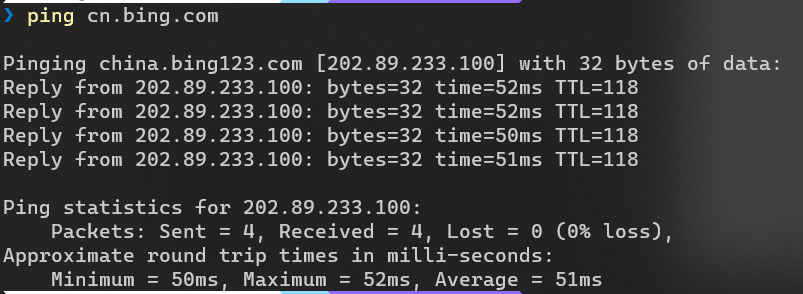
\includegraphics[width=0.6\textwidth]{ping.png}
\end{figure}

为了灵活调整工作量,我们要求ping的输出至少能够包含时延的部分。


\subsubsection{nslookup}

nslookup是一个用于DNS解析的命令行工具。我们实现该程序,可以更详细地测试DNS的实现。
nslookup命令的典型输出如图\ref{fig:nslookup}所示。

\begin{figure}[htb]
	\centering
	\caption{nslookup}
	\label{fig:nslookup}
	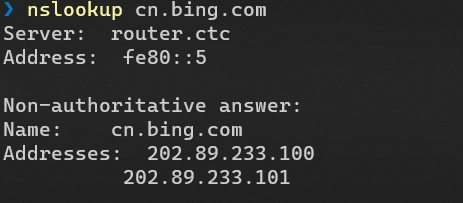
\includegraphics[width=0.6\textwidth]{nslookup.png}
\end{figure}

为了灵活调整工作量,我们要求nslookup的输出至少包含解析结果的IP地址。


\subsubsection{TCP echo server}

TCP echo server是一个基于TCP的回声服务器。我们实现该程序,来综合验证服务器侧的Socket接口是否能正常工作。
TCP echo server的典型功能是将收到的数据原路发回给客户端。如果我们实现了Epoll机制,我们将会同时提供使用和未使用该机制的TCP echo server。
我们的TCP echo server的实现将会输出接收到的数据,以及接收到的数据的长度。

\subsection{(可选)epoll系统调用}

现代Linux内核为了实现高性能的网络操作、避免过大的系统调用开销、防止轮询浪费CPU时间,实现了epoll。它采用
事件驱动的模型,有效地解决了高并发下的性能问题。在连接数目增多时显现出了明显的性能优势。

在客观条件允许的情况下,我们会为xv6内核实现这一机制,并评估其性能。


\section{外围工作}

xv6源自Unix V6,它有较长的历史。它的代码中,一些实现较为原始,另一些实现则偏离了当前的软件工程上的最佳实践。
为了更好地完成本项目,一些辅助工作需要在主要任务之外完成。这些工作对网络子系统的运行效率和开发难度可能有显著的积极影响,
但并非必须,因此我们会根据客观条件的限制来选择性地完成。由于我们具有相关经验,因此这些辅助工作的工作量和难度处在可控的范围内。
这些辅助工作包括:

\begin{itemize}
	\item Buddy\cite{peterson1977buddy}/Slab\cite{bonwick1994slab}内存分配系统
	\item 进程子系统对POSIX Signals的支持
	\item 进程间通信机制
	\item newlib作为用户态C标准库的移植
\end{itemize}

\section{测试方法}

为了测试该网络子系统的正常运行,我们主要通过网络应用程序的输出来间接推断。

这大致包括以下内容:

\begin{itemize}
	\item \textbf{ping}: 是否能够正常地对特殊的IP地址(如localhost:127.0.0.1)收发ICMP报文、是否能对任意IP地址手法ICMP报文、DNS的解析是否正常。
	\item \textbf{nslookup}:是否能够正常地对特殊的域名(如localhost)解析、是否能对任意域名进行解析。
	\item \textbf{TCP echo server}:能否正常处理连接的请求、能否正常处理收到的数据并输出相应信息、能否正确地发回收到的信息。
\end{itemize}

如果我们对IPv6进行了支持,在上述测试中,我们会对使用IPv4地址的情形和IPv6地址的情形进行分别测试。

\section{性能基准测试}

为了评估我们的网络子系统实现的性能,我们将会对其进行性能基准测试。具体而言,我们会对在JOS/xv6上实现了上述功能的开源项目以及我们的实现进行性能的对比测试。
这将会包含以下内容:

\begin{itemize}
	\item \textbf{ping}:ping的时延
	\item \textbf{TCP echo server}:TCP echo server的吞吐量
\end{itemize}

如果实现了Epoll机制,我们会进一步对比采用和未采用Epoll机制的TCP echo server的运行效率。

\clearpage
\section*{参考文献}
\addcontentsline{toc}{part}{参考文献}

\bibliographystyle{unsrt}
\bibliography{reference}


\end{spacing}

\end{document}